\section{System Architecture}
This work focuses on an HPC accelerator architecture that combines general-purpose RISC-V cores and an analog coprocessor consisting of one or more analog MVM arrays in a single \emph{tile}.
This architecture takes full advantage of the open RISC-V ISA to integrate the analog coprocessor as a functional unit for each core invoked through ISA extensions.
Treating the analog arrays as discrete functional units allows the system to effectively use a specialized computational kernel accelerator due to the low overhead of data movement into and out of the analog arrays.

Each tile also contains local SRAM, in the evaluated implementation using hardware-managed caches for programming simplicity; however, using a mix of caches and software-managed scratchpad memories is an important potential architectural optimization.
Tiles are connected through a high-bandwidth mesh router, and are for programmer simplicity fully cache coherent.

Notably, the proposed tile architecture looks similar to digital RISC-V accelerators such as the Tensix cores in the Tenstorrent Grayskull. \cite{10820793} %cite from last year
In both instances, specialized functional units---matrix and vector FPU for Tensix, analog arrays for the proposed tile---are tightly integrated with scaler compute cores to enable fine-grained offload of more complex operations.
The proposed architecture makes several simplifications to reduce design complexity, specifically the use a cache for local storage rather than the specialized circular buffer SRAM, using a single general RISC-V core rather than specialized \textit{baby cores}, and as discussed in the next section, the communication between the analog arrays and general-purpose core using local scratchpad rather than a specialized packer and unpacker cores.
It is likely that many of the Tensix core optimizations would benefit the proposed analog-enabled core; however the increase in design and programming model complexity makes these optimizations beyond the scope of this initial study.

\begin{figure}[ht]
    \centering
    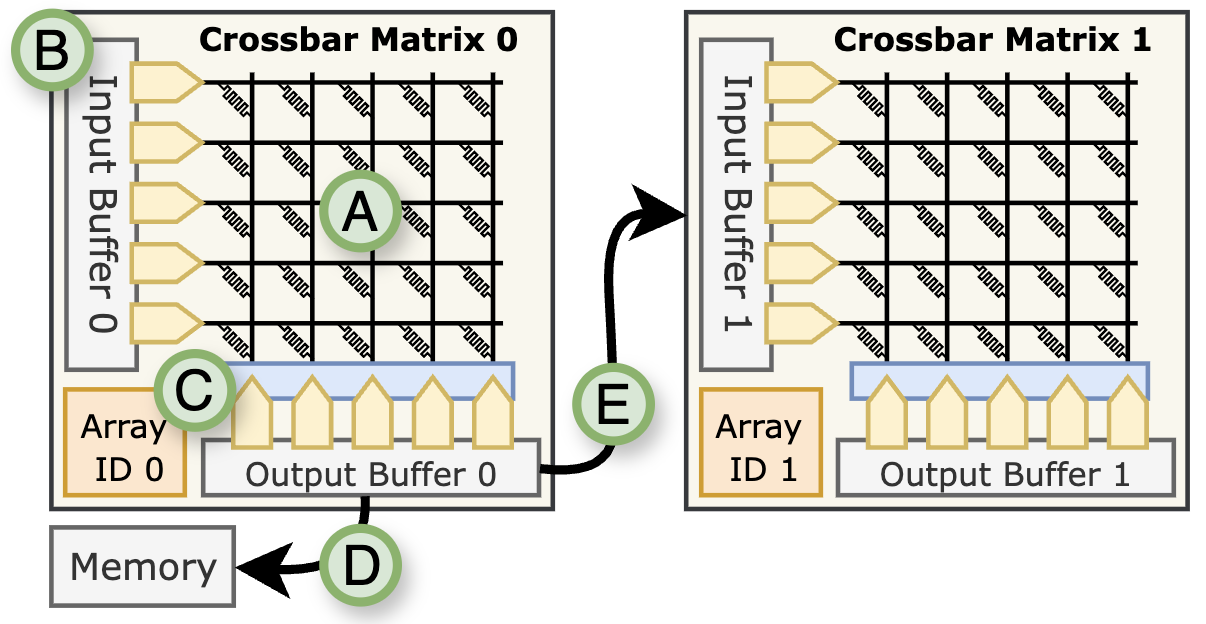
\includegraphics[scale=0.42]{figures/compute_arrays.png}
    \caption{RoCC Commands in action}
    \label{fig:rocc_commands}
\end{figure}

\subsection{Analog Coprocessor}
The analog coprocessor is organized into one or more compute arrays, each serving as an independent processing unit for analog operations.
Every compute array contains three ISA-visible components:
\begin{itemize}
    \item \textbf{Analog array}---contains the programmed analog conductance values. 
        Importantly, in this work we do not optimize the implementation for programming the analog arrays as such work requires substantial device-specific details and for program-once applications is not a major factor in overall system performance.
    \item \textbf{Input buffer}---holds the input operand vector for the MVM operation.
        These values are converted into analog voltages by the array's digital-to-analog converters (DACs).
    \item \textbf{Output buffer}---holds the result of the analog computation as digital values after conversion by analog-to-digital converters (ADCs).
\end{itemize}

For the CPU to coprocessor interface we adopt the conventions of the Rocket Custom Coprocessor (RoCC) interface. \cite{Asanović:EECS-2016-17}
The RoCC interface is an extension point that lets custom coprocessors integrate directly with the CPU pipeline.
Five core instructions form the basis of accelerator and are represented in Figure~\ref{fig:rocc_commands}. 
As noted above, rather than passing individual values in the instructions, we opt to use the local SRAM for passing data between the core and coprocessor.
This is a significant advantage when using multiple arrays per coprocessor.
By allowing each coprocessor to individually perform memory accesses through a dedicated memory port---shared among all arrays within the coprocessor---the RISC-V CPU can perform other operations rather than individually writing operands through the RoCC interface.

This design choice also leads to a uniform structure for the ISA extensions.
Each instruction uses \textit{rs1} to specify the array within the coprocessor, and \textit{rs2} to specify the starting address of the memory access for the given operation.
Finally, since we are focusing on an HPC accelerator, we use a floating point interface for the coprocessors under the assumption that each ISA-visible array is actually multiple arrays using a scheme for combining outputs as in prior work~\cite{8416841,10.1145/3581784.3607077}.
In systems tailored for neural network inference operations, these operations would likely need to be performed on the general purpose CPU rather than in dedicated hardware within the coprocessor.

\begin{figure}[ht]
    \centering
    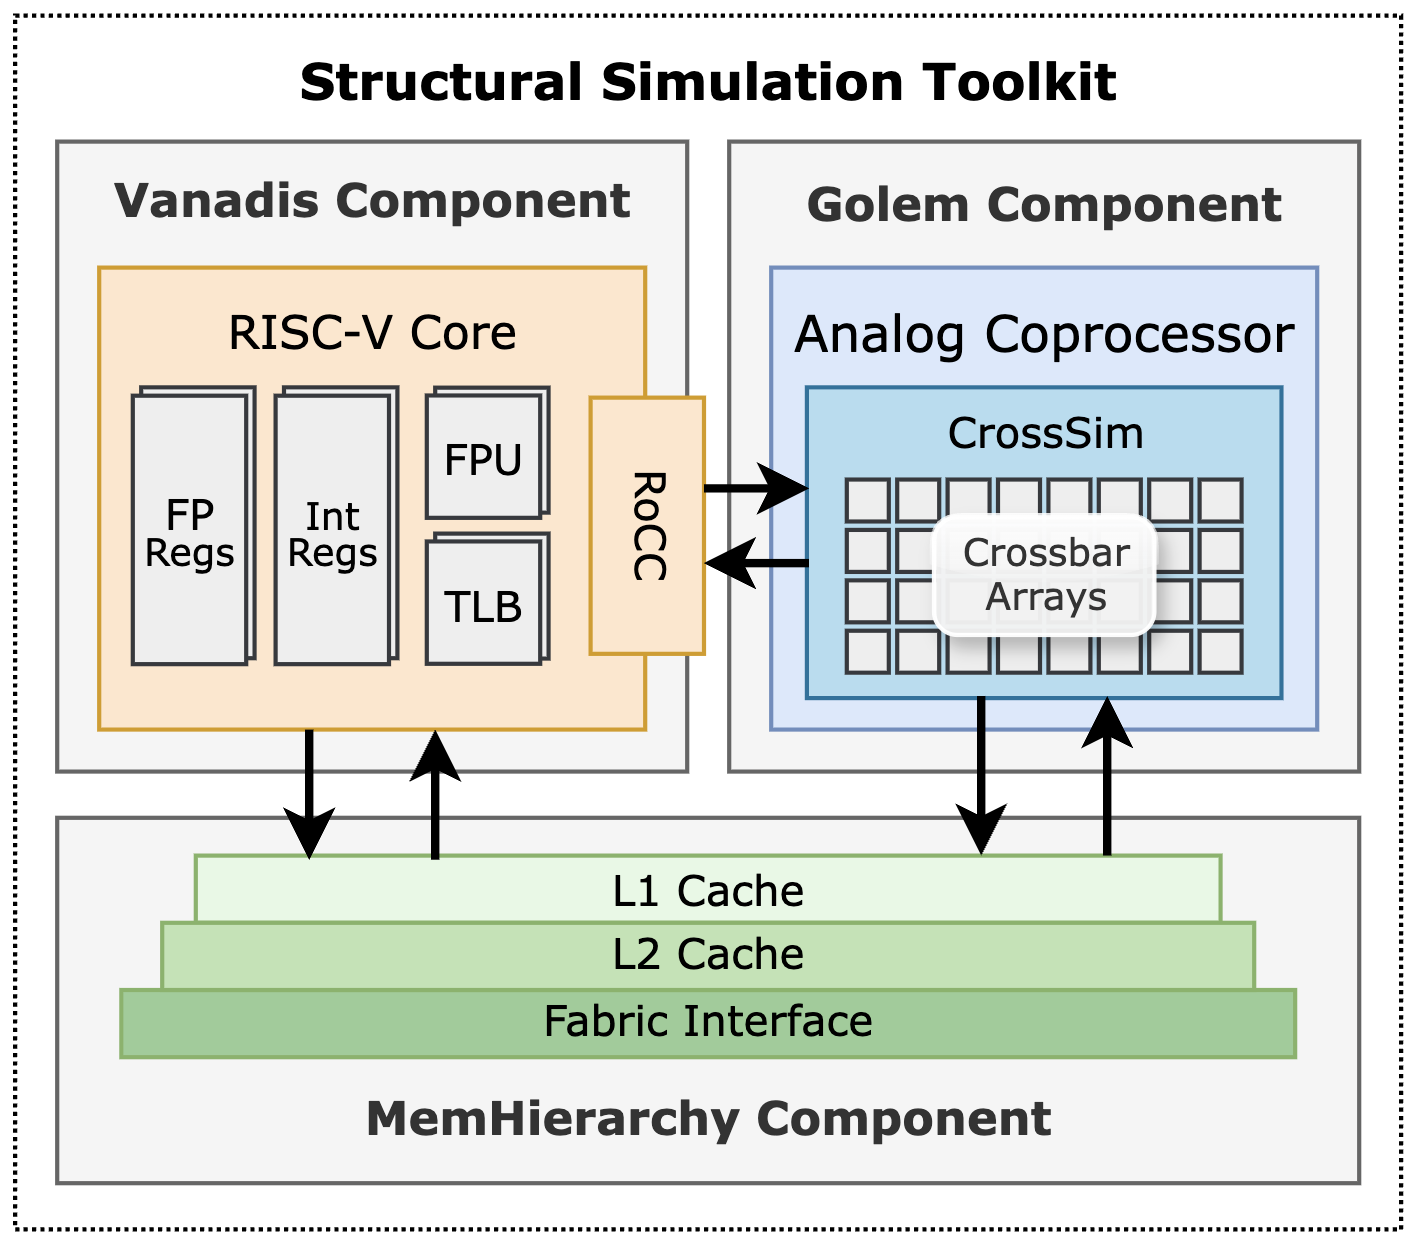
\includegraphics[scale=0.30]{figures/arch_detailed.png}
    \caption{System Architecture showing component integration in SST}
    \label{fig:architecture}
\end{figure}


A typical analog computation begins with the processor configuring a compute array using \textit{mvm.set} (Symbol A in Figure~\ref{fig:rocc_commands}), followed by \textit{mvm.l} (Symbol B) to load the operand vector.
Once both the matrix and vector are staged locally, the \textit{mvm} instruction (Symbol C) initiates computation within the analog array, producing results in the output buffer.
These results can either be stored back to memory with \textit{mvm.s} (Symbol D) or forwarded directly to another array using \textit{mvm.mv} (Symbol E) to enable multiple-stage processing without additional memory traffic.
Cascading MVM operations across multiple arrays within the same tile allows for complex transformations to be executed entirely without off-chip memory accesses, keeping all intermediate data at the source of computation.

% \subsection{Memory Hierarchy}
% The memory hierarchy is designed to sustain high-throughput demands of tiles while preserving full cache coherence across the mesh.
% Each tile's private L1 data and instruction caches have access to the execution pipeline, where operand fetch and result writebacks are issued in parallel. 
% A shared L2 cache connects to the rest of the system through a high-radix mesh router with dedicated ports for each tile.



\subsection{System Simulation Model}
The architecture in Figure~\ref{fig:architecture}, is realized by three specialized SST components: \textit{Vanadis}, \textit{MemHierarchy}, and \textit{Golem} .
\textit{Vanadis} models an out-of-order RISC-V core with configurable reorder buffers, pipeline widths, functional units, and load/store queues.
\textit{MemHierarchy} implements the private L1 and shared L2 caches, a directory-based MESI protocol, and DRAM controllers linked through a high-radix mesh router.
The mesh provides dedicated ports for every core, accelerator, and memory controller enabling multi-core computation. 
\textit{Golem} models the analog accelerator, including crossbars and buffers.
Together, these components enable full-system execution of RISC-V binaries while tracking pipeline behavior, performance and utilization in a HPC-class models.

% The accelerator has DMA 

% Are RoCC instructions blocking/non blocking?
% How does RoCC integrate with vanadis timing model?
% How are DMA requests handled-immediate or queued?
